\section{Extensions}
\label{kvdirect:sec:extensions}

\subsection{CPU-based Scatter-Gather DMA}

For 64B DMA operations, PCIe has a 29\% TLP header and padding overhead (\S \ref {kvdirect:sec:challenge}), and the DMA engine may not have enough parallelism to saturate the PCIe Bandwidth-Delay Product (BDP) with small TLPs. The PCIe root complex in the system supports larger DMA operations, up to 256 bytes of TLP payload. In this case, the TLP header and padding overhead is only 9\%, and the DMA engine has enough parallelism (64) to saturate the PCIe link with 27 ongoing DMA reads. To batch DMA operations on the PCIe link, the CPU can be utilized to perform scatter-gather (Figure \ref {kvdirect:fig:sg-arch}). First, the NIC DMA sends addresses to a request queue in host memory. The host CPU polls the request queue, performs random memory accesses, places data into a response queue, and writes an MMIO doorbell to the NIC. Then, the NIC extracts data from the response queue via DMA.

\begin{figure}[htbp]
		\centering
		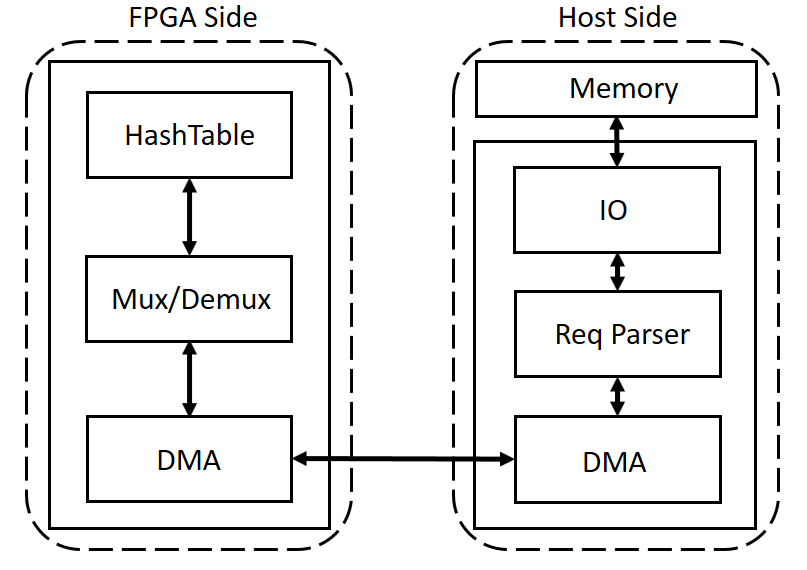
\includegraphics[width=0.6\textwidth,page=1]{scatter_gather.PNG}
		\caption{Scatter-gather architecture.}
		\label{kvdirect:fig:sg-arch}
\end{figure}

Figure \ref {kvdirect:fig:scatter-gather} shows that, compared to the CPU bypass method, the throughput of CPU-based scatter-gather DMA is improved by 79\%. Besides the CPU overhead, the main disadvantage of CPU-based scatter-gather is the additional latency. To batch 256 DMA operations per doorbell from the CPU to the NIC, it takes 10 $\mu$s to complete. The total latency for the NIC to access host memory using CPU-based scatter-gather is about 20 $\mu$s, nearly 20 times higher than direct DMA.

\begin{figure}[htbp]
	\centering
	\subfloat[Read operations.\label{kvdirect:fig:sge-read}]
	{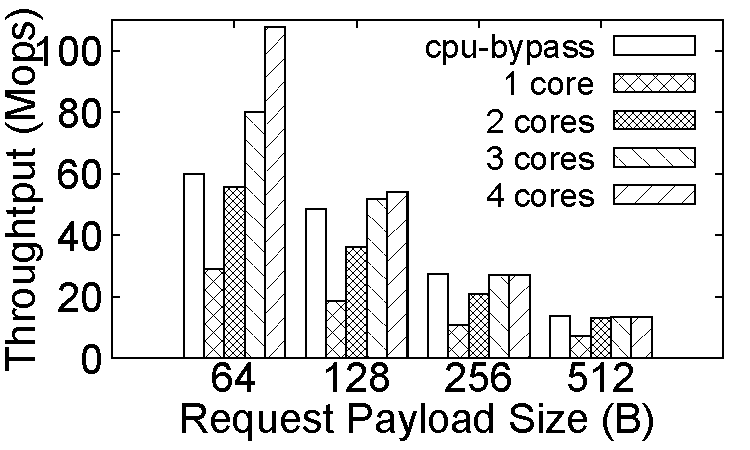
\includegraphics[width=.5\textwidth,page=1]{sg-read.pdf}}
	\subfloat[Write operations.\label{kvdirect:fig:sge-write}]
	{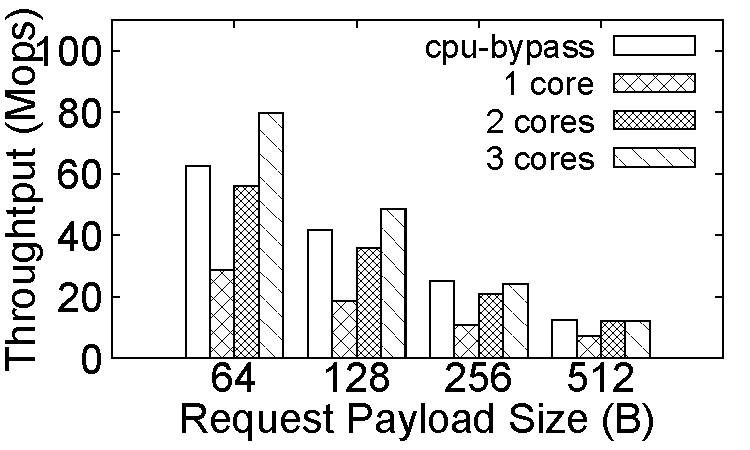
\includegraphics[width=.5\textwidth,page=1]{sg-write.pdf}}
	\caption{Scatter-gather performance.}
	\label{kvdirect:fig:scatter-gather}
\end{figure}

\subsection{Single-Host Multi-NIC}
\label{kvdirect:sec:multi-nic}

The primary use case of KV-Direct is to enable remote direct key-value access without CPU overhead on the server. In some cases, it may be necessary to build a dedicated key-value store with maximum throughput per server. Through simulation, \cite {li2016full} showed the possibility of achieving one billion key-value operations on a single server with four (currently unavailable) 60-core CPUs. As shown in Table \ref{kvdirect:tab:kvs-compare}, with 10 KV-Direct NICs on the server, it is easy to achieve one billion key-value op/s performance using a commercial server.

As shown in Figure \ref{kvdirect:fig:photo}, the server consumes 357 watts of power (measured at the wall) to achieve 1.22~Gop/s GET or 0.61~Gop/s PUT performance.

\begin{figure}[htbp]
	\centering
	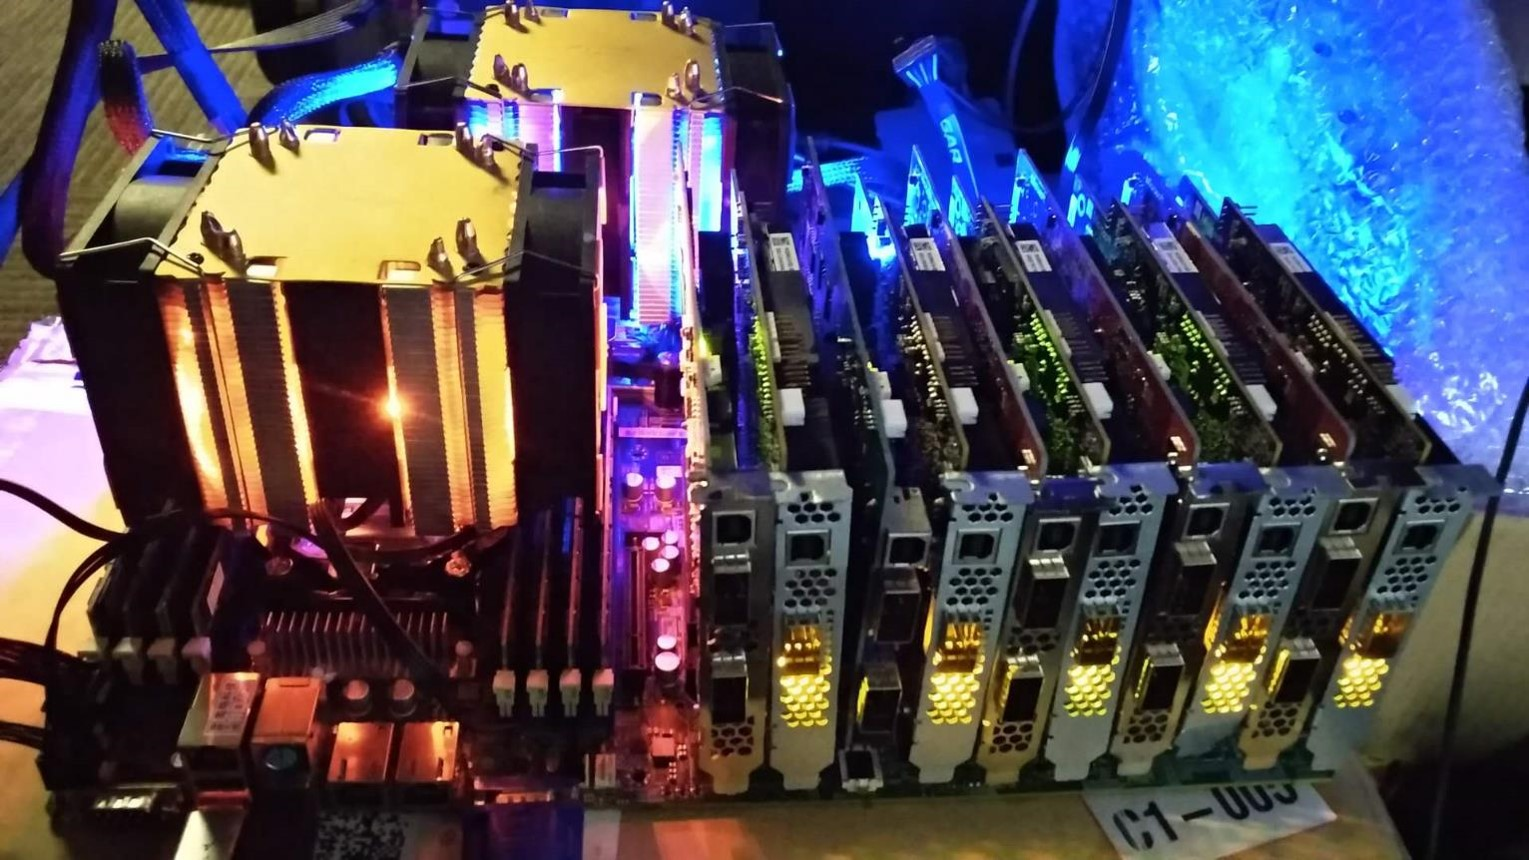
\includegraphics[width=0.9\textwidth]{figure/kvdirect_photo.jpg}
	\caption{10-card KV-Direct system achieving 1.22 billion key-value operations per second at 357 watts power consumption.}
	\label{kvdirect:fig:photo}
\end{figure}

To saturate the 80 PCIe Gen3 lanes of two Xeon E5 CPUs, the motherboard of the benchmark server was replaced with a SuperMicro X9DRX+-F motherboard with 10 PCIe Gen3 x8 slots, the PCIe topology is shown in Figure \ref{kvdirect:fig:pcie_topology}.

\begin{figure}[htbp]
	\centering
	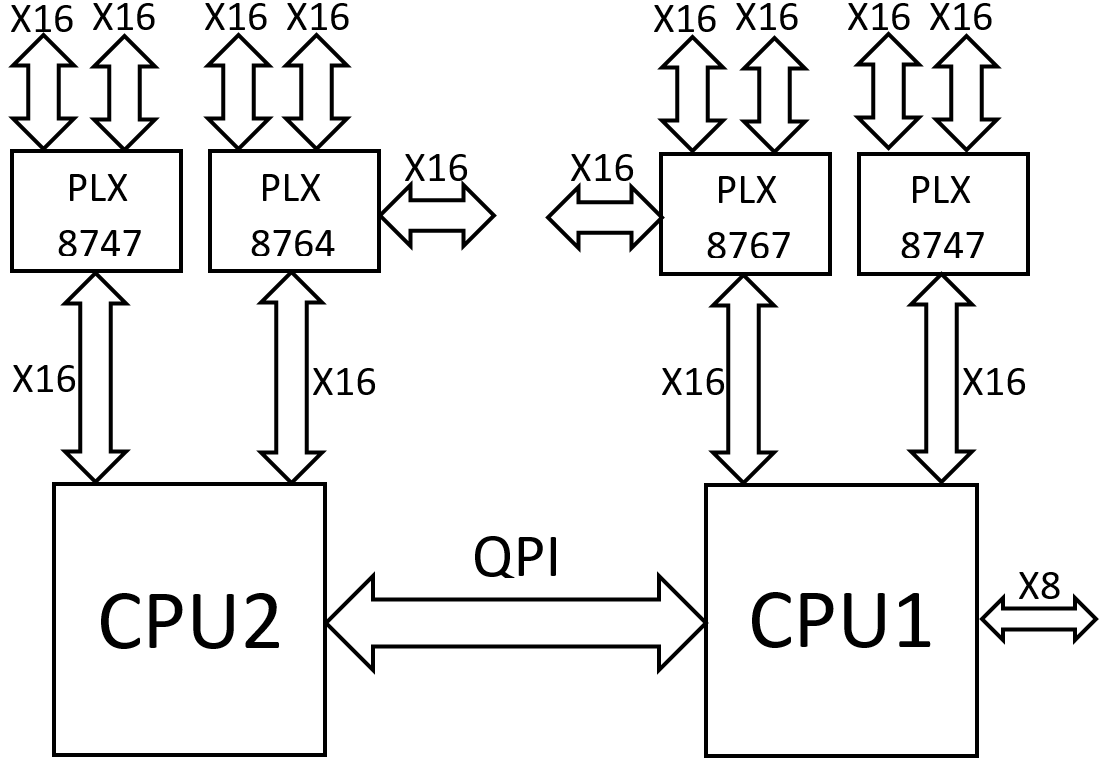
\includegraphics[width=0.5\textwidth]{figure/pcie_topology.PNG}
	\caption{PCIe topology of the 10-card KV-Direct system.}
	\label{kvdirect:fig:pcie_topology}
\end{figure}

Each of the 10 programmable network cards on each slot is connected using a PCIe x16 to x8 converter, with only one PCIe Gen3 x8 link enabled on each network card, so the throughput of each network card is lower than that shown in Figure \ref {kvdirect:fig:ycsb-tput}.
Each network card has an exclusive memory area in the host memory and provides disjoint key partitions.
Multiple network cards encounter the same load imbalance problem as multi-core key-value storage implementations.
Fortunately, for a small number of partitions (such as 10), load imbalance is not important \cite {lim2014mica,li2016full}. Under the YCSB long-tail workload, the average load of the network card with the highest load is 1.5 times, and the load increase of very popular keys is provided by the out-of-order execution engine (\S \ref {kvdirect:sec:ooo}).
In contrast, to achieve performance matching with 240 CPU cores, the load of the hottest CPU core will be 10 times the average.
Figure \ref {kvdirect:fig:multiple-nics} shows that the throughput of KV-Direct is almost linearly related to the number of network cards on the server.

\begin{figure}[htbp]
	\centering
	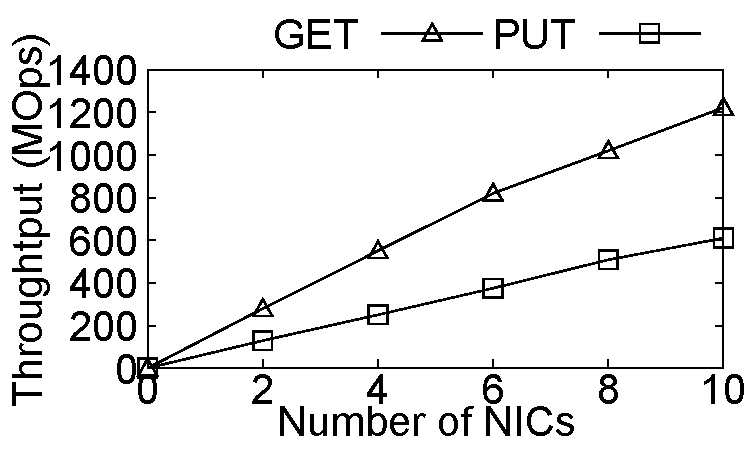
\includegraphics[width=0.5\textwidth,page=1]{multi_nic.pdf}
	\caption{Performance scalability of multiple network cards on a single machine.}
	\label{kvdirect:fig:multiple-nics}
\end{figure}

\subsection{SSD-based Durable Storage}
\label{sec:durable-storage}

Data will be lost after power failure in memory-based data structure storage. For persistence, this section implements persistent key-value storage using SATA SSD. Since the number of SSDs on the server is limited, and the operating system and applications also run on the SSD, the key-value storage needs to share the SSD hardware with the operating system and applications.
For this, the SSD provides two access interfaces: block storage and key-value storage. Similar to the dedicated memory space used by memory key-value storage, key-value storage is also located in a dedicated block storage space.
The CPU needs two ways to access block storage: one is to access the block device through the operating system's storage protocol stack, and the other is to bypass the operating system and directly access it through the user-mode fast interface.
Since the operating system itself and many software run on block storage, it is necessary to maintain the compatibility of the first traditional access method.
Storage performance-sensitive applications use the runtime library provided in this paper to access block storage through the second method.

\begin{figure}[htbp]
	\centering
	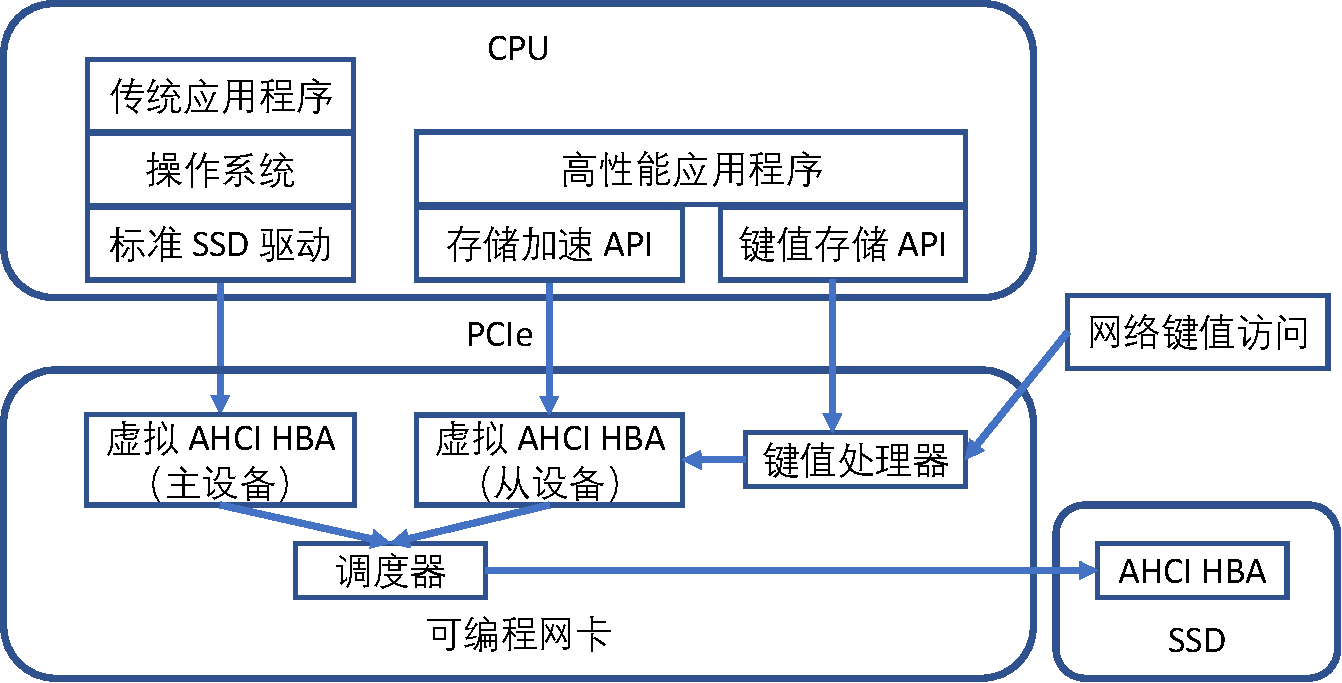
\includegraphics[width=0.9\textwidth]{ssd.pdf}
	\caption{SSD persistent storage architecture.}
	\label{kvdirect:fig:ssd}
\end{figure}

As shown in Figure \ref{kvdirect:fig:ssd}, the programmable network card virtualizes the SSD into two virtual AHCI HBA devices.
The scheduler inside the programmable network card virtualizes the data plane of the storage hardware (such as the 32 request slots of SATA and the request queue of NVMe) into two logical storage devices.
The control registers of the storage hardware (such as PCIe configuration registers) are transparently passed to the main logical storage device and managed by the original operating system.
The secondary logical storage device has no control plane, only a data plane, and can only perform data read and write operations, and cannot perform management operations.
The above storage virtualization architecture does not require the programmable network card to manage the control plane, simplifying the design of the scheduler; and it maintains compatibility with the original storage device driver and operating system.
As shown in Figure \ref{kvdirect:fig:ssd-benchmark}, the sequential access throughput of the original operating system and software after storage virtualization through the main logical storage device has not changed significantly. The delay has increased from about 30 $\mu$s to about 60 $\mu$s, which is the overhead of the programmable network card forwarding. Due to the increase in latency, the throughput of single-threaded random access (4K block size) has also decreased. When 64 threads are randomly accessed, because SATA only has 32 request slots, that is, only 32 read and write requests can be performed in parallel, the throughput is limited by the average delay of the request.

\begin{figure}[htbp]
	\centering
	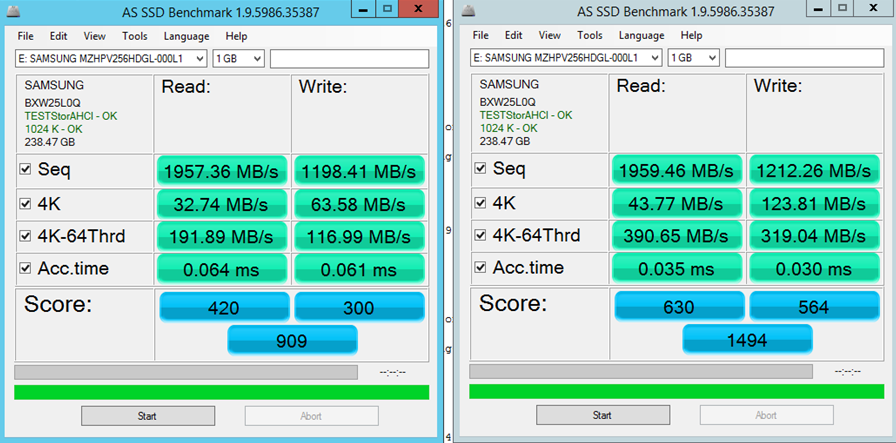
\includegraphics[width=0.8\textwidth]{storahci.png}
	\caption{Performance evaluation of SSD virtualization. The left figure is the result of the original operating system and SSD performance test program after storage virtualization. The right figure is the performance test result of this SSD without using storage virtualization.}
	\label{kvdirect:fig:ssd-benchmark}
\end{figure}

In order to provide an efficient block device access interface, this section uses the PCIe I/O pipeline of Chapter \ref{chapter:clicknp} to allow applications to directly access the programmable network card through the storage acceleration API, bypassing the operating system and driver.
The storage acceleration API can access any storage block on the SSD, and it is the responsibility of the application to avoid conflicts with the file system of the operating system. Usually, the application creates a large file to reserve storage space.
Experiments show that with only a single CPU thread, the storage acceleration API can fully utilize the sequential read and write throughput of about 2 GB/s on the SSD and the random read and write throughput of about 50 K times per second with a 4K block size.
The traditional operating system storage protocol stack requires 8 CPU threads to fully utilize the throughput of random read and write with a 4K block size.
In order to provide persistent key-value storage, the key-value processor is connected to the slave device of virtual storage, and treats virtual storage as a large piece of memory for reading and writing.
This paper does not optimize for the read and write characteristics of SSD, which will be future work.

\subsection{Distributed Key-Value Storage}

In distributed key-value storage, we assume that each host is both a client using key-value storage and can allocate some memory resources as a key-value server. Each key-value pair needs to be replicated on multiple server nodes to provide high availability and improve the performance of key-value access. Traditional key-value storage services simply select servers based on the hash value of the key. However, not every host accesses each key with the same probability. For example, in graph computing, if a host is responsible for processing a vertex, then the probability of accessing the key-value corresponding to the vertex will be higher than other hosts. At this time, the key-value pair of the vertex is best stored on the host to take advantage of locality to accelerate access.

Distributed storage systems need to decide on which hosts each key-value pair is replicated. Read operations only need to read the nearest replica. Write operations need to be synchronized to all replicas through the master node. If there are too many replicas, the master node synchronizing write operations to each replica will become a bottleneck. To balance the load between the master node and each replica node, the number of replicas depends on the read-write ratio. Assuming the ratio of read and write operations is $R$, and $R$ is much greater than 1 \footnote{In write-intensive workloads, if there is only one master node, not making any replicas is obviously the most performance optimal. For high availability, it may be necessary to limit the minimum number of replicas.}. It can be derived that when the load of the master node is equal to that of the replica node, the number of replicas is approximately $\sqrt{R}$. Compared with a single replica, the load of read operations is reduced by about $\sqrt{R}$ times; compared with replication to each host, the load of write operations is reduced by about $\sqrt{R}$ times.

After deciding on the number of replicas, the next question is to select the most frequently read hosts for replication. This paper maintains an approximate counter for read and write times for each key in the programmable network card of the master node \footnote{The approximate counter is to save storage space. For example, the approximate count is represented by an 11-bit significand and a 5-bit exponent floating point number. Each time you access, the significand is incremented with a probability of one in the power of 2.}. When write operations are synchronized to each replica, the master node summarizes the read times of all replicas. The optimal number of replicas can be calculated based on the ratio of read and write times, and the number of replicas can be increased or decreased when it differs significantly from the current number of replicas, so that the replicas are stored on several nodes with the most read times. To prevent the master node from not being able to respond to a large number of read requests in a timely manner due to scarce write operations, the replica node can also actively report to the master node after receiving a large number of read requests.

Another problem is that the access frequency of some keys may be so high that the throughput of a single machine may become a bottleneck. For example, the serial number generator in distributed transactions, the access counter of popular network resources, and the lock of shared resources require high-throughput single-key atomic operations. Recent works such as NetCache \cite{netcache-sosp17}, NetChain \cite{jin2018netchain} use programmable switches as caches to achieve higher single-key read and write performance than a single host, but they are still limited by switch performance.

This paper proposes that with multi-master replication, single-key read and write performance can scale with the number of hosts and ensure strong consistency. The mechanism to ensure consistency is the token ring, at any time there is only one node holding the token processing write operations. The token is passed in order on the ring formed by each master node and carries the current latest value. The key to the token ring's ability to improve single-key performance is that read and write operations and many atomic operations are associative. For example, multiple write operations can be reduced to the last write operation; multiple atomic addition and subtraction operations can be reduced to one atomic addition and subtraction operation; compare and swap atomic operations are more complex, but multiple operations can also be reduced to a lookup table of size not exceeding the number of atomic operations. Therefore, when a node does not hold a token, it records the received operations in the buffer and reduces these operations. When the token arrives, the node can quickly execute the reduced operation based on the latest value, and send the updated value with the token to the next node. After that, the node replays the operations in the buffer and returns the result of each operation to the client. Theoretical analysis shows that when requests arrive evenly at each master node, the system's throughput and average delay increase linearly with the number of master nodes. The worst delay is the time it takes for the token ring to turn around. Since the operations in the buffer are reduced, the processing delay of each node is bounded, and the time for the token ring to turn around is also bounded. The size of the request buffer required for each master node is equal to the product of the worst delay and network bandwidth. The overhead of the token ring is a packet that is constantly passed in the network, even if there are no read and write requests, the token has to be constantly passed in the network.

The actual key-value storage system has more than one frequently accessed key. The network overhead of setting a token for each key is too high, so this paper uses one token to serve all keys. However, waiting for all keys to be processed and then sending all updated key-value pairs in a concentrated manner will bring higher latency. Assuming that the keys accessed over a period of time are random, that is, most key-value operations involve non-repetitive keys. At this time, the size of the key-value update carried by the token is proportional to the number of key-value operations in the buffer, and the time to transmit these key-value updates is no longer bounded, so the request delay will tend to infinity as the load factor approaches 1. For this reason, this paper pipelines key-value processing and transmission between adjacent master nodes. The master node organizes the key-value operations in the buffer into a priority queue sorted by key in ascending order, and the key-value updates are also sent in ascending order of keys, and the token indicates the end of the key-value update sequence. When the master node receives the update of key $K$, the key-value operations in the buffer that do not exceed $K$ can be processed and sent to the next master node along the token ring. In this way, multiple master nodes on the token ring can concurrently process different keys, that is, the master nodes closer to the direction of token passing process smaller keys. Theoretical analysis shows that when the keys of the requests follow a uniform distribution and the requests arrive evenly at each master node, the request delay is still bounded, regardless of the load factor, and is only slightly higher than the delay in the single-key situation.

\section{Discussion}
\label{kvdirect:sec:discussion}

\subsection{Network Interface Card Hardware of Different Capacities}
\label{kvdirect:sec:different-nic}

The goal of KV-Direct is to offload significant workloads (key-value access) using existing data center hardware, rather than designing special hardware to achieve maximum key-value storage performance. Programmable network cards usually contain a limited amount of DRAM for buffering and connection state tracking. Large DRAM is expensive in terms of chip size and power consumption.

Even if future network cards have faster or larger onboard memory, under long-tail workloads, the load distribution design of this paper (\S \ref {kvdirect:sec:dram-cache}) still shows higher performance than simple partition design. Keys are unified according to the capacity of the network card and host memory.
Table \ref {kvdirect:tab:optimal-load-dispatch} shows the optimal load distribution ratio for long-tail workloads with 1 billion keys, different network card DRAM and PCIe throughput, and different network card and host memory size ratios.
If the network card has faster DRAM, more load is dispatched to the network card. A load distribution ratio of 1 indicates that the behavior of the network card memory is exactly the same as the cache of the host memory.
If the network card has larger DRAM, slightly less load is dispatched to the network card.
As shown in Table \ref {kvdirect:tab:optimal-load-dispatch-throughput}, even if the size of the network card DRAM is only a small part of the host memory, the throughput gain is significant.

\begin{table}[htbp]
	\centering
	\caption{Optimal load distribution ratio for long-tail workloads under different network card DRAM / PCIe throughput (vertical) and network card / host memory size ratio (horizontal).}
	\label{kvdirect:tab:optimal-load-dispatch}
	\small
	\begin{tabular}{|l|r|r|r|r|r|r|}
		\hline
		& 1/1024 & 1/256 & 1/64 & 1/16 & 1/4 & 1 \\
		\hline
		1/2  & 0.366 & 0.358 & 0.350 & 0.342 & 0.335 & 0.327 \\
		\hline
		1    & 0.583 & 0.562 & 0.543 & 0.525 & 0.508 & 0.492 \\
		\hline
		2    & 0.830 & 0.789 & 0.752 & 0.718 & 0.687 & 0.658 \\
		\hline
		4    & 1     & 0.991 & 0.933 & 0.881 & 0.835 & 0.793 \\
		\hline
		8    & 1     & 1     & 1     & 0.995 & 0.937 & 0.885 \\
		\hline
	\end{tabular}
\end{table}


\begin{table}[htbp]
	\centering
	\caption{Relative throughput of load dispatch compared to simple partitioning. Row and column titles are the same as Table \ref{kvdirect:tab:optimal-load-dispatch}.}
	\label{kvdirect:tab:optimal-load-dispatch-throughput}
	\small
	\begin{tabular}{|l|r|r|r|r|r|r|}
		\hline
		& 1/1024 & 1/256 & 1/64 & 1/16 & 1/4 & 1 \\
		\hline
		1/2 & 1.36	& 1.39	& 1.40	& 1.37	& 1.19	& 1.02 \\ 
		\hline
		1	& 1.71	& 1.77	& 1.81	& 1.79	& 1.57	& 1.01 \\
		\hline
		2	& 2.40	& 2.52	& 2.62	& 2.62	& 2.33	& 1.52 \\
		\hline
		4	& 3.99	& 4.02	& 4.22	& 4.27	& 3.83	& 2.52 \\
		\hline
		8	& 7.99	& 7.97	& 7.87	& 7.56	& 6.83	& 4.52 \\
		\hline
	\end{tabular}
\end{table}


The out-of-order execution engine (\S \ref {kvdirect:sec:ooo}) can be applied to various applications that need to hide latency, and this paper hopes that future RDMA network cards can support more powerful atomic operations.

In a 40~Gbps network, network bandwidth limits the key-value throughput of non-batch transfers, so this paper uses client batching. With higher network bandwidth, the batch size can be reduced, thereby reducing latency. In a 200~Gbps network, the KV-Direct network card can reach 180~Mop/s without batch transfer.

KV-Direct utilizes widely deployed programmable network cards and FPGA implementation \cite{putnam2014reconfigurable,caulfield2016cloud}. FlexNIC \cite {kaufmann2015flexnic,kaufmann2016krishnamurthy} is another promising architecture of programmable network cards with reconfigurable match-action tables (RMT) \cite {bosshart2013forwarding}.
NetCache \cite {netcache-sosp17} implements key-value caching in programmable switches based on RMT, showing the potential to build KV-Direct in network cards based on RMT.

\subsection{Performance Impact on Real-world Applications}

When KV-Direct is applied to end-to-end applications, backend computation shows potential performance improvement. In PageRank \cite{page1999pagerank}, each edge traversal can be achieved through a single key-value operation, thus KV-Direct supports 1.22G TEPS on a server with 10 programmable network cards. In contrast, GRAM \cite{wu2015g} supports 250M TEPS per server, constrained by interleaved computation and random memory access.

KV-Direct supports user-defined functions and vector operations (Table \ref{kvdirect:tab:kv-operations}), which can further optimize PageRank by offloading client computation to hardware. Similar parameters apply to the parameter server \cite{li2014scaling}. This paper hopes that future work can leverage hardware-accelerated key-value storage to improve the performance of distributed applications.

\subsection{Stateful Processing in Programmable Network Cards}
\label{kvdirect:sec:stateful-nic}

The ClickNP architecture of Chapter \ref{chapter:clicknp} is more suitable for stateless or simple state pipeline data packet processing, but it is inadequate for processing based on connection state or application layer requests. For example, the scheduler and hash table in the Layer 4 load balancer application are tightly coupled with the application logic, making it difficult to scale to a large number of concurrent connections, and the code maintainability is not strong. In fact, a lot of time was spent in the development process to solve deadlock problems.

KV-Direct proposes a new architecture for stateful processing. The fundamental difference between KV-Direct and traditional general-purpose processor architectures lies in the separation of control, computation, and memory access. In traditional processors, computation and memory access share the same instruction stream, so for serial programs alternating between computation and memory access, the computation and memory access logic often need to wait for each other, resulting in neither the computation nor memory access throughput being fully utilized. KV-Direct uses separate control instruction streams, computation instruction streams, and memory access instruction streams, and exploits the parallelism between KV operations with an out-of-order execution engine, allowing computation and memory access to be fully pipelined. Developers need to divide the request processing process into several stages alternating between computation and memory access, and abstract the request processing process into a state machine. The control instruction stream manages the state of the request and dispatches the next stage task to the computation or memory access components. After a stage of the task is completed by the computation or memory access components, it returns to the controller.

\begin{figure}[htbp]
	\centering
	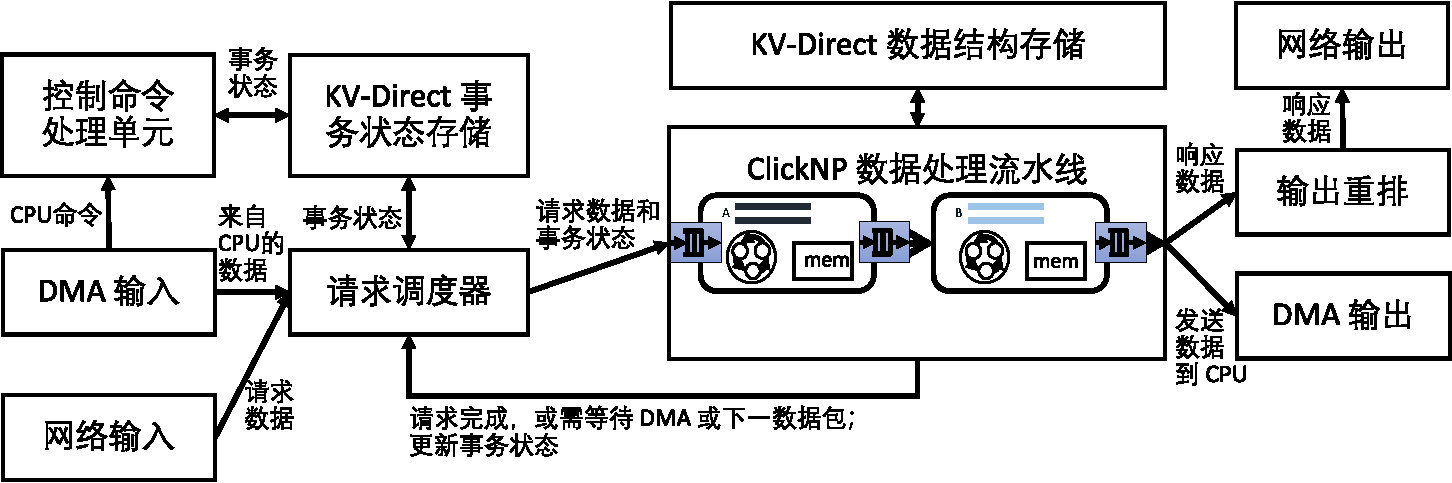
\includegraphics[width=1.0\textwidth]{../figures/kvdirect_arch.pdf}
	\caption{Application layer architecture based on KV-Direct for programmable network cards.}
	\label{arch:fig:kvdirect_arch_application}
\end{figure}

The stateful processing architecture based on KV-Direct is shown in Figure \ref{arch:fig:kvdirect_arch_application}. Transactions represent dependencies, such as a connection in stateful network processing, an application layer HTTP request split across multiple packets, or operations on the same key in key-value storage. Different requests within the same transaction need to be processed in sequence, while requests in different transactions can be processed concurrently. To hide latency and maximize concurrent processing capability, the request scheduler looks up the transaction number corresponding to the request from the transaction state key-value storage based on KV-Direct, and queues the requests of the transactions being processed. The data processing pipeline based on ClickNP processes according to the request data and transaction state, and may query other data structures (such as memory allocation tables, host virtual address mapping tables, firewall rule tables, routing tables, etc.) during the processing. If the request processing is completed, the response data enters the output rearrangement module, rearranges the order of responses to meet the consistency requirements of transaction processing (for example, requests from different transactions also need to respond in the order of arrival), and finally outputs to the network. If the processing of the request still depends on the next packet or data DMA from the host memory, in order not to block the data processing pipeline, the request will return to the scheduler, waiting for the dependent operation to complete before proceeding to the next stage of processing.

The KV-Direct architecture can serve as the basis for many programmable network card applications, such as the stateful network functions in Chapter \ref{chapter:clicknp} (such as Layer 4 load balancers) and the scalable RDMA in Chapter \ref{chapter:socksdirect}.

\subsection{Extending from Key-Value to Other Data Structures}
\label{kvdirect:sec:data-structure}

KV-Direct implements a hash table data structure for key-value mapping. Key-value storage systems represented by Redis \cite{redis} in data centers also support secondary indexes, ordered key-value sets, message queues, and other data structures. The essential features of these more complex data structures are stateful processing within programmable network cards (Section \ref{kvdirect:sec:stateful-nic}).

For message queues, the advantage of FPGA processing is fast centralized coordination. In the producer-consumer model, the message queue needs to distribute the producer's messages to each consumer, which is a centralized FIFO abstraction. Due to the limited single-core processing capability of the CPU, parallel or distributed message queues often need to sacrifice some consistency \footnote{Consistency refers to the first-come, first-served order feature} to improve performance scalability. However, the clock frequency of FPGA hardware logic is sufficient to handle requests at 100 Gbps line speed, without sacrificing consistency.

In the message queue based on KV-Direct, messages are stored in a circular linked list composed of fixed-size buffers. The use of a circular linked list facilitates the allocation of new fixed-size buffers when space is insufficient, and also facilitates the recycling of buffers that have been idle for a long time. For the producer-consumer model, a head pointer is maintained for all producers, and a tail pointer is maintained for all consumers. For the publisher-subscriber model, a head pointer is maintained for all publishers, and a tail pointer is maintained for each subscriber, allowing different subscribers to receive messages at different speeds.

In the secondary index, requests are queued in the request scheduler according to the primary index, and the metadata matching the primary index of the secondary index is obtained using the standard KV-Direct method. The metadata is stored in the transaction status storage as a cache. Then a new request is generated for the secondary index query, which is queued in the request scheduler according to the merged primary and secondary index. When processing this request, the corresponding metadata is taken from the transaction status storage and a second DMA query is initiated. In addition, another complexity of the secondary index compared to the single-level index is that the secondary index may often need to change the size of the hash table when adding or deleting elements, thus requiring rehashing, during which the operations corresponding to the primary index need to be suspended and wait. The advantage of using FPGA to handle secondary indexes is the fine-grained memory access latency hiding, such as other secondary indexes can operate during the rehashing of a certain secondary index.
